\newpage
\section{Durchführung}
\subsection{Aufgabenteil a)}
Die Aufnahme der Kennlinien für das Ablesen des Sättigungsstrom erfolgt durch einen Versuchsaufbau nach Abbildung (\ref{fig:aufbau1}), 
jedoch wird hier auf den XY-Schreiber verzichtet.

\begin{figure}
    \centering
       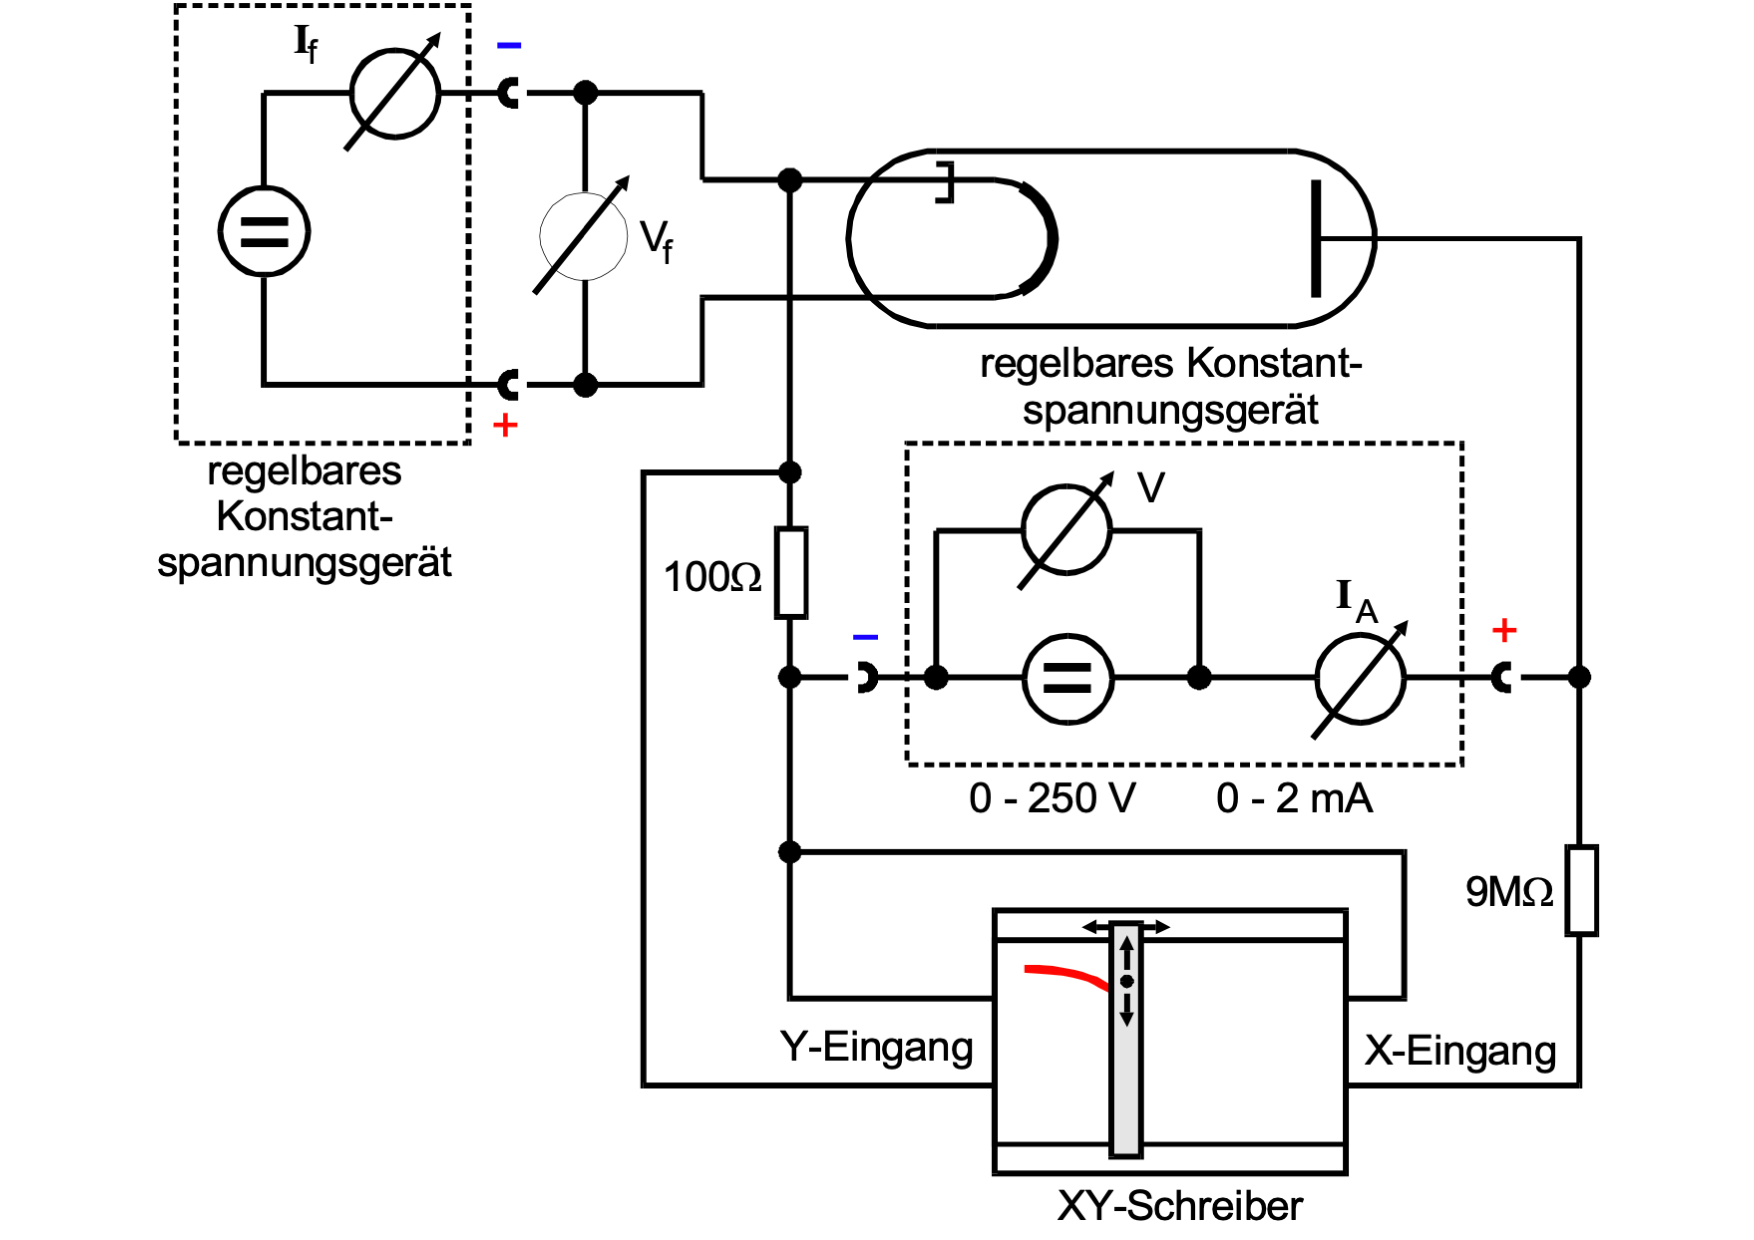
\includegraphics[height=5cm]{aufbau1.pdf}
       \caption{Potentialtopf-Modell (Quelle: \cite{V504}).}
       \label{fig:aufbau1}
\end{figure}

\noindent
Bei maximalem Heizstrom (2,5A bei 5,5V) wird die Messreihe gestartet, 
indem bei einer Saugspannung von 0V bis 250V in Intervallen gemessen und jeweils der Anodenstrom in Abhängigkeit von der Saugspannung notiert wird.
Dieser Vorgang wird noch vier mal wiederholt, wobei der Heizstrom pro Messung um 0,1A verringert wird.
Die Messwerte sind in Tabelle ??%(\ref{tab:a})
einzusehen.

\subsection{Aufgabenteil c)}
Um das Anlaufstromgebiet der Diode zu untersuchen, wurde zunächst der Versuch nach (\ref{fig:aufbau2}) umgebaut, 
da nun ein Nanoamperemeter benötigt wird.

\begin{figure}
    \centering
       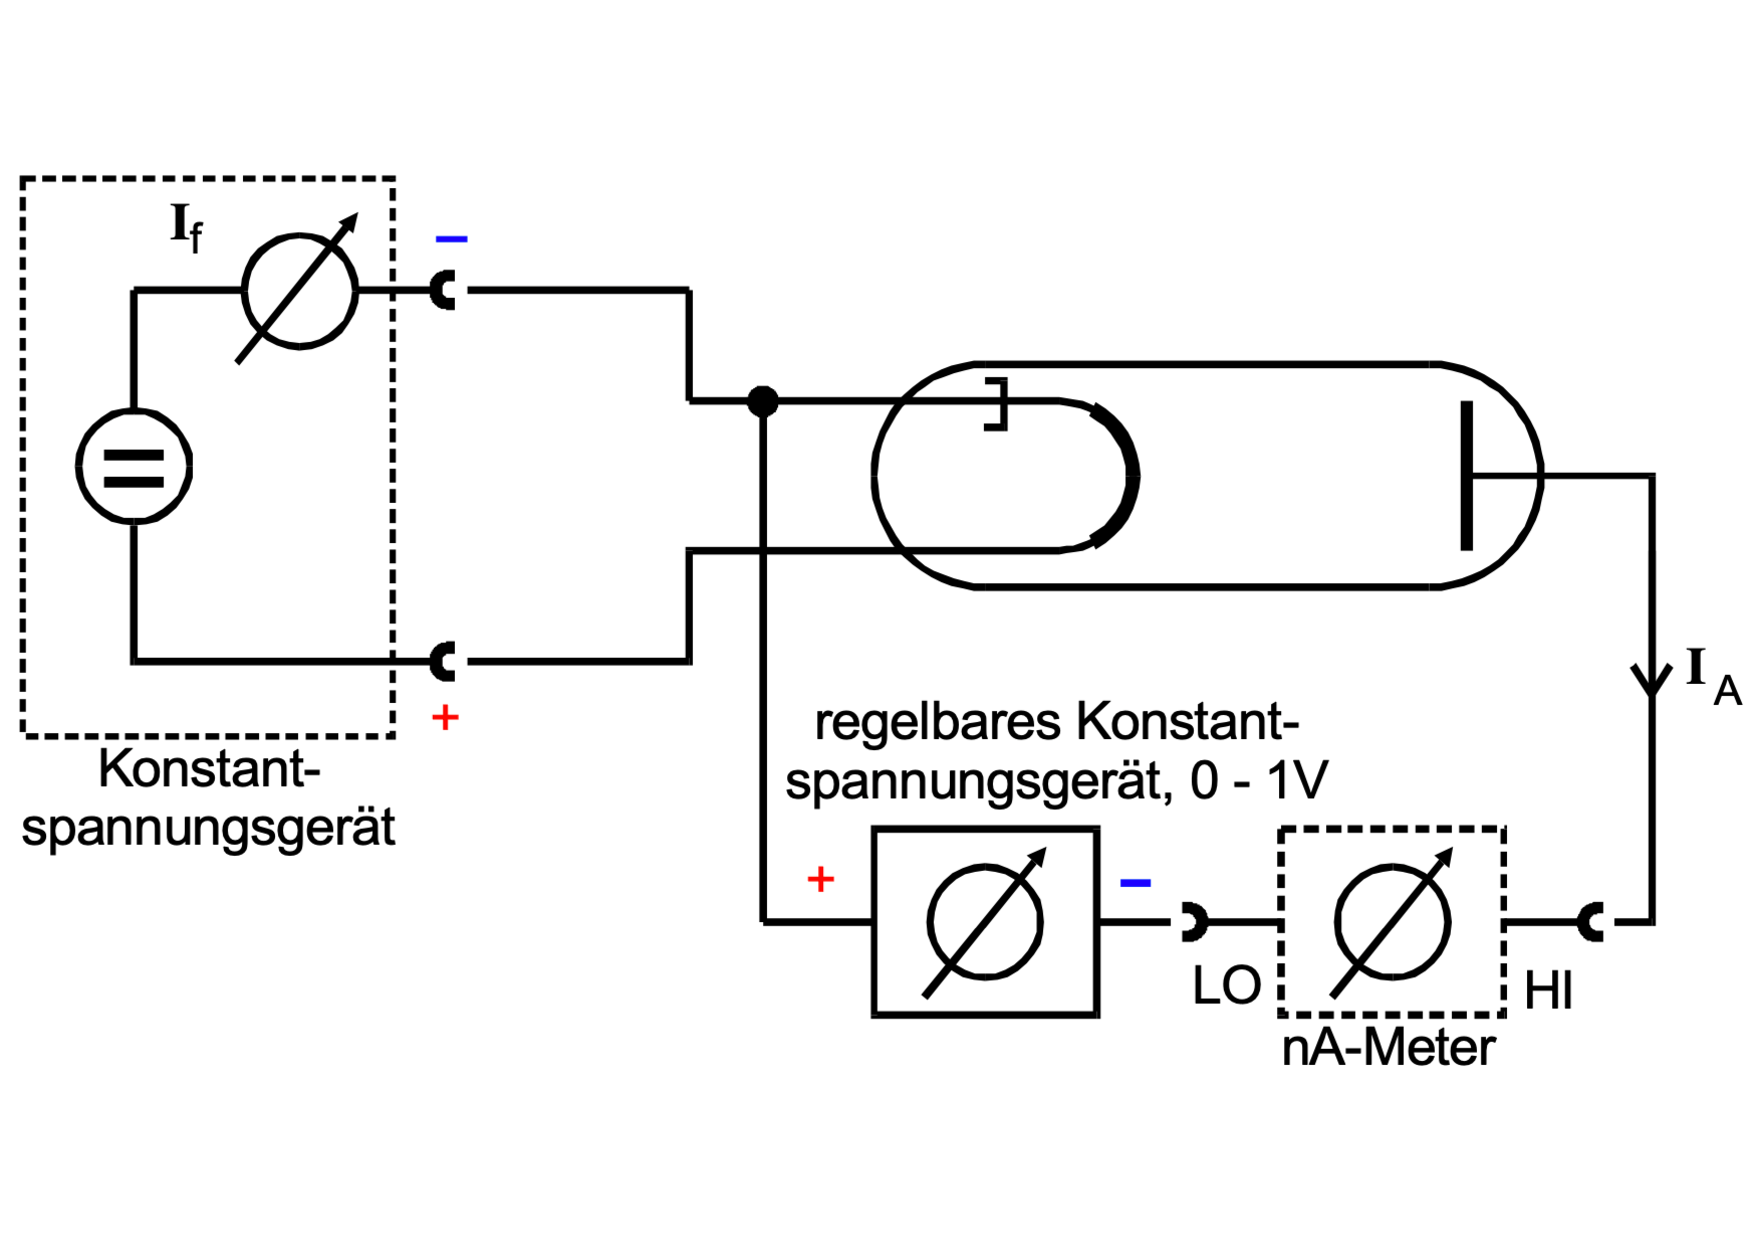
\includegraphics[height=5cm]{aufbau2.pdf}
       \caption{Potentialtopf-Modell (Quelle: \cite{V504}).}
       \label{fig:aufbau2}
\end{figure}

\noindent
Sodann wird wieder bei maximalem Heizstrom (2,5A bei 5,5V) die Saugspannung von 0V bis 1V Intervallmäßig erhöht 
und jeweils der Anodenstrom in Abhängigkeit von der Saugspannung notiert.
Die Dabei aufgenommenen Messwerte befinden sich in Tabelle ??%(\ref{tab:c})
.